- how numerics are used to solve Equations from Theory section

\subsection{Smoothed Particle Hydrodynamics}
- before finite difference schemes with spherical coordinates
- spherical coordinates bad for collisions


Smoothed Particle Hydrodynamics is a numerical simulation method first introduced by \cite{Monaghan_1977} in 1977. It is a Lagrangian particle method and as such often used when the geometry of the underlying problem makes it difficult to apply Eulerian grid-based methods like finite difference schemes. Although SPH is most often used to model liquids, it is possible to add physical models for solids as well.

- explanations apply to Miluphcuda

Miluphcuda is a smoothed particle hydrodynamics code that has been developed over several years at the University of Tuebingen by Christoph Schaefer and others. Its general use is well documented in \cite{Schaefer_2016}.

\subsubsection{Main SPH concepts}
A SPH simulation is composed of many individual SPH particles. Each particle moves through space with a velocity $\vec{v}$ and a mass m. In contrast to particle methods used for N-body simulations or molecular dynamics, SPH particles carry information about continuous variables such as the density $\rho$ or energy e. The particles only act as computational points at which equations from hydrodynamics/continuum mechanics such as the Euler or Navier-Stokes Equations are evaluated. Solving such equations comes down to converting partial differential equations to a system of first order ordinary differential equations in time.

\begin{equation} \label{eq:ode}
    \frac{d\vec{y}}{dt} = f(t, \vec{y}(t), A_1, ..., A_n)
\end{equation}

In equation \ref{eq:ode} $\vec{y}$ is a vector of quantities to be projected forward in time and $A_1$ through $A_n$ are quantities that are calculated at every step. Once $A_1$ through $A_n$ are known for every particle and the right hand side of quation \ref{eq:ode} can be evaluated, standard integrators such as Runge-Kutta or Predictor-Corrector methods are used to update $\vec{y}$.

To calculate a quantity A at a particle location, SPH uses a weighted average of A over all particles in the neighborhood:

\begin{equation}
    A(\vec{r}\,) \approx \int A(\vec{r}\,') W(\vec{r} - \vec{r}\,', h) \mathrm d\vec{r}\,'
\end{equation}

\subsubsection{Smoothing kernel}
The kernel function $W(|\vec{r} - \vec{r'}|$, h) at the particle location $\vec{r}$ depends upon the distance to the other particles and a specific length h called the smoothing length. Most kernels used today have compact support within a radius of h. To ensure normalization of the kernel

\begin{equation} \label{eq:kernel_normalization}
    \int W(\vec{r} - \vec{r}\,', h)\mathrm d\vec{r}\,' = 1
\end{equation}

- Smoothing kernel image: \ref{fig:smoothing_kernel}

\begin{figure}[H]
    \centering
    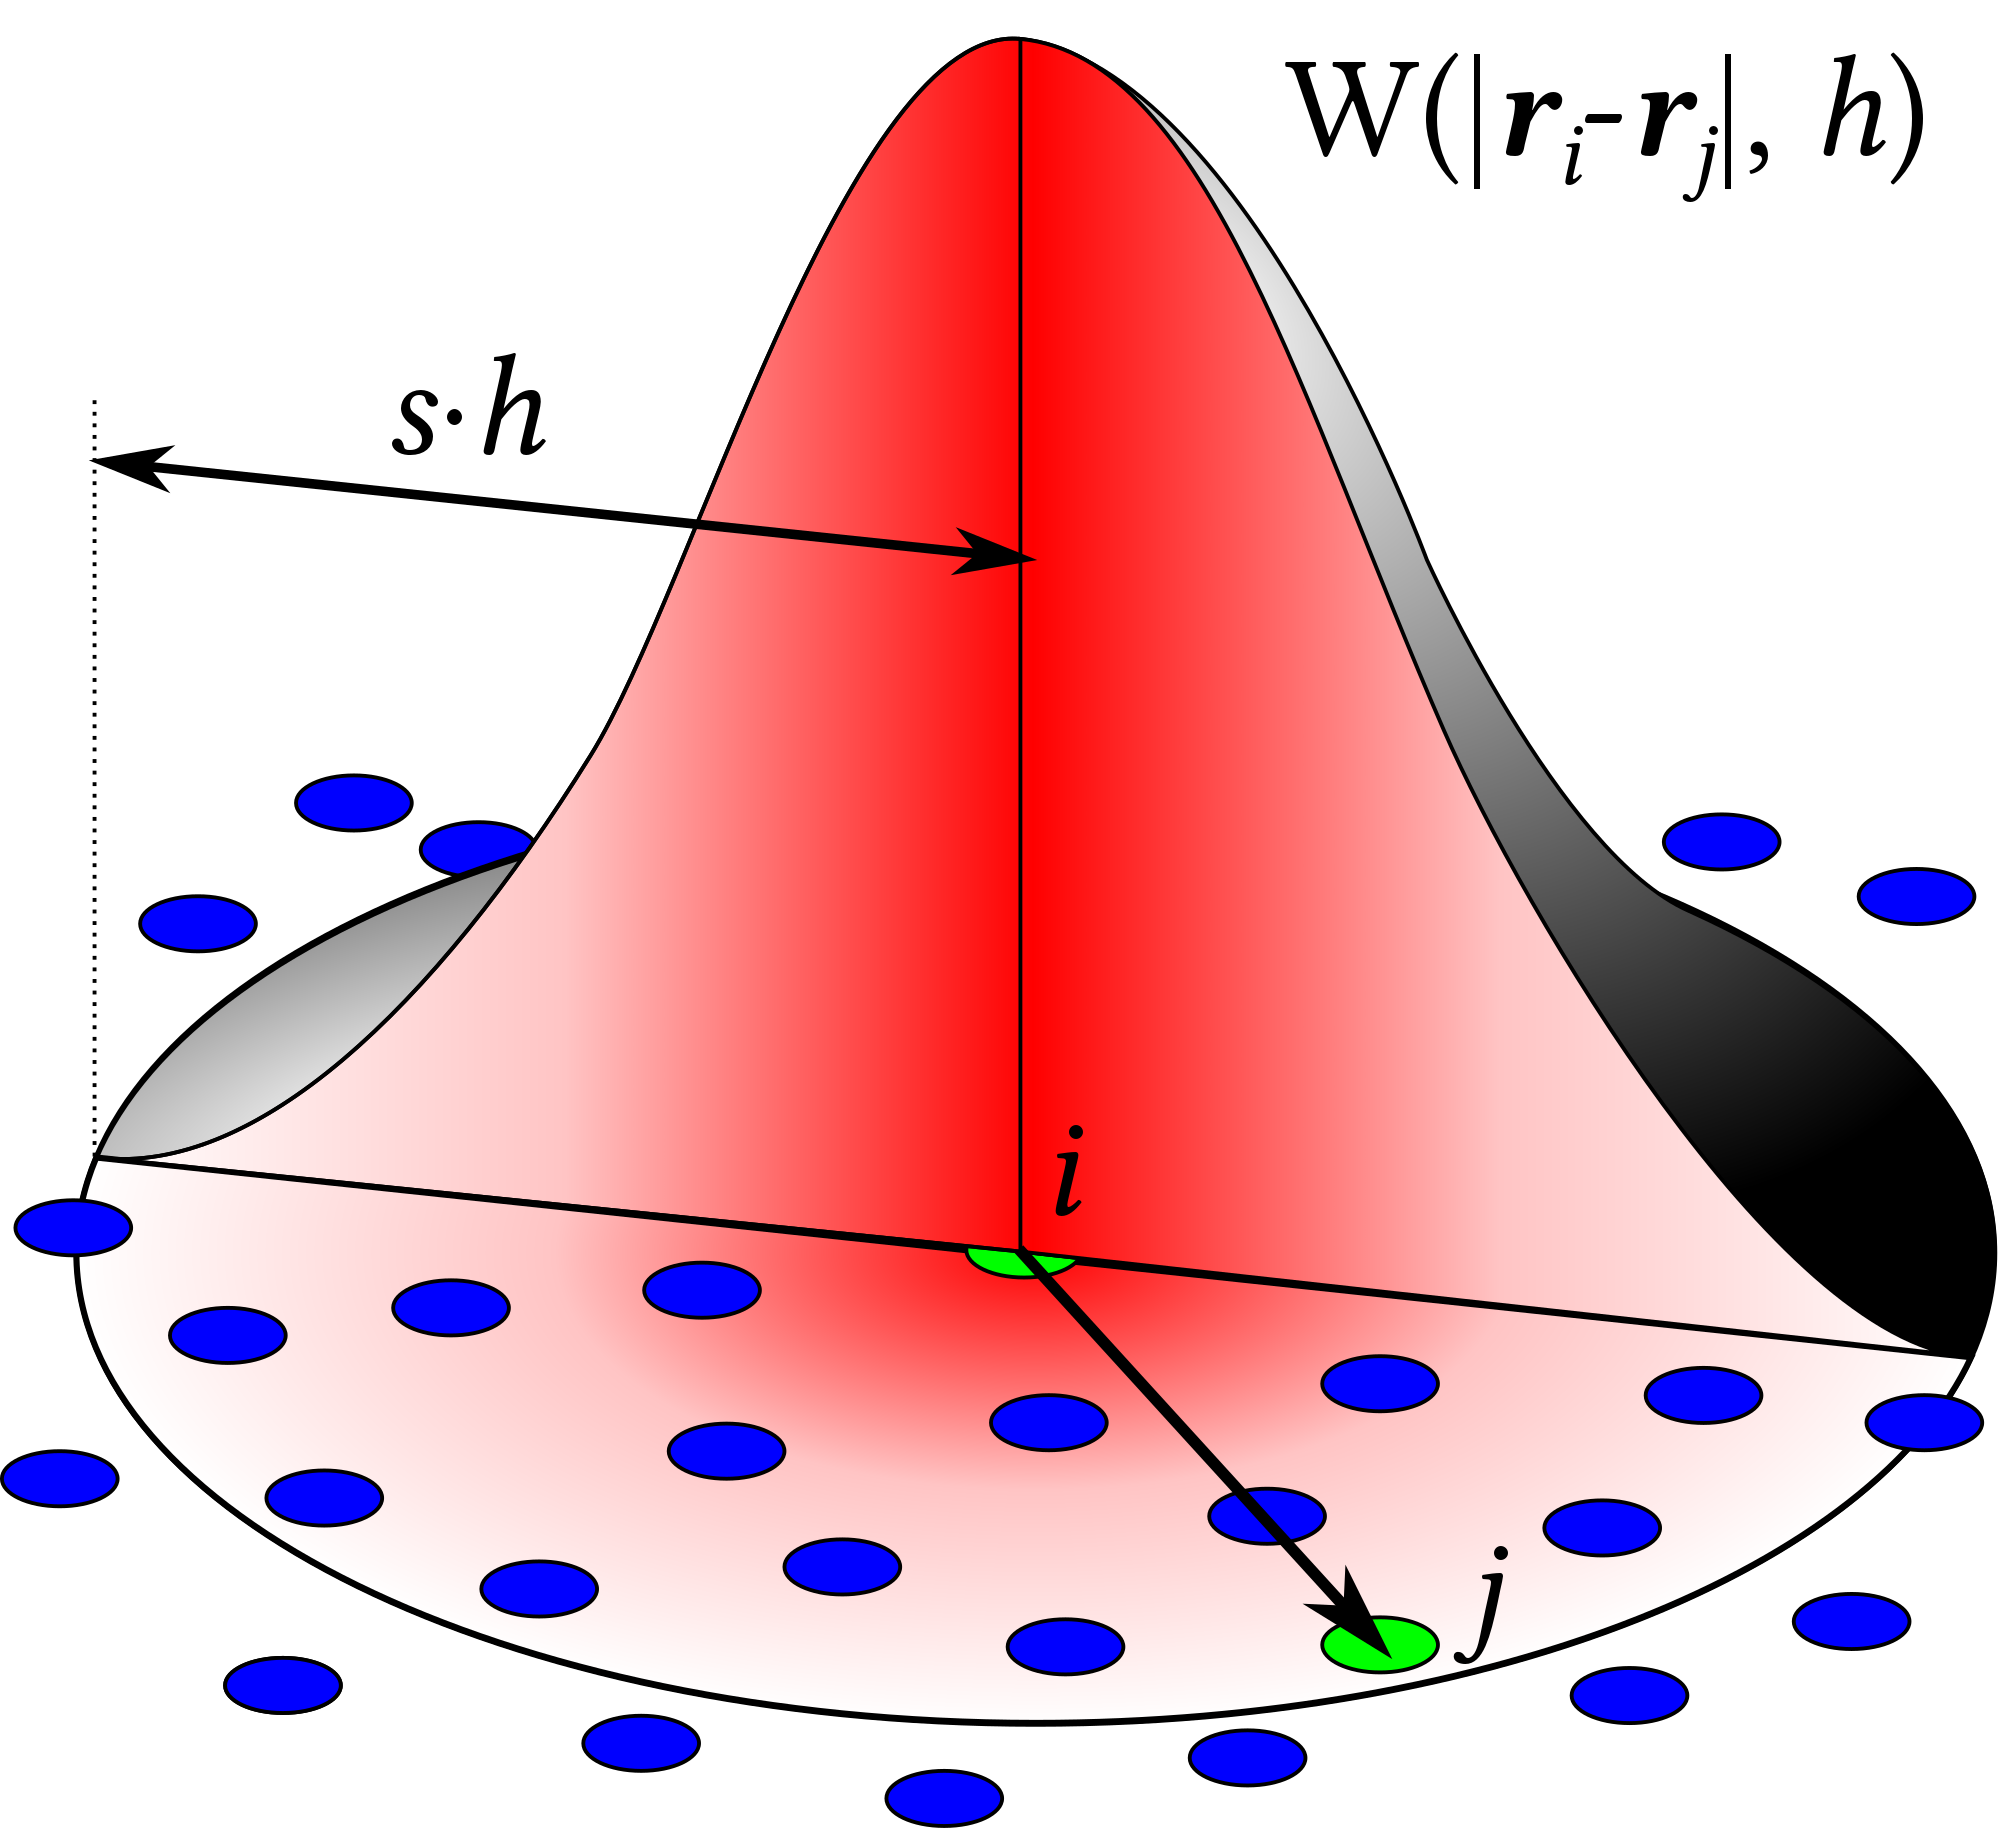
\includegraphics[width=0.5\textwidth]{smoothing_kernel.png}
    \caption{Kernel function \cite{image:smoothing_kernel}}
    \label{fig:smoothing_kernel}
\end{figure}

\subsubsection{Smoothing length}
- can be variable -> great strength of SPH
- material density and h have to fit together

\subsubsection{Artificial viscosity}
- what it is
- why it is needed

\subsubsection{Time Integration}

\subsection{Initial conditions}
\subsubsection{Particle setup}
- Target basalt halfsphere \\
- Impactor aluminium sphere \\
- resolution bound to variable smoothing length \\
- Uniform macro structure but random micro structure to avoid \\
- seagen \cite{github:SEAGen} used to create initial conditions

\begin{figure}[H]
    \centering
    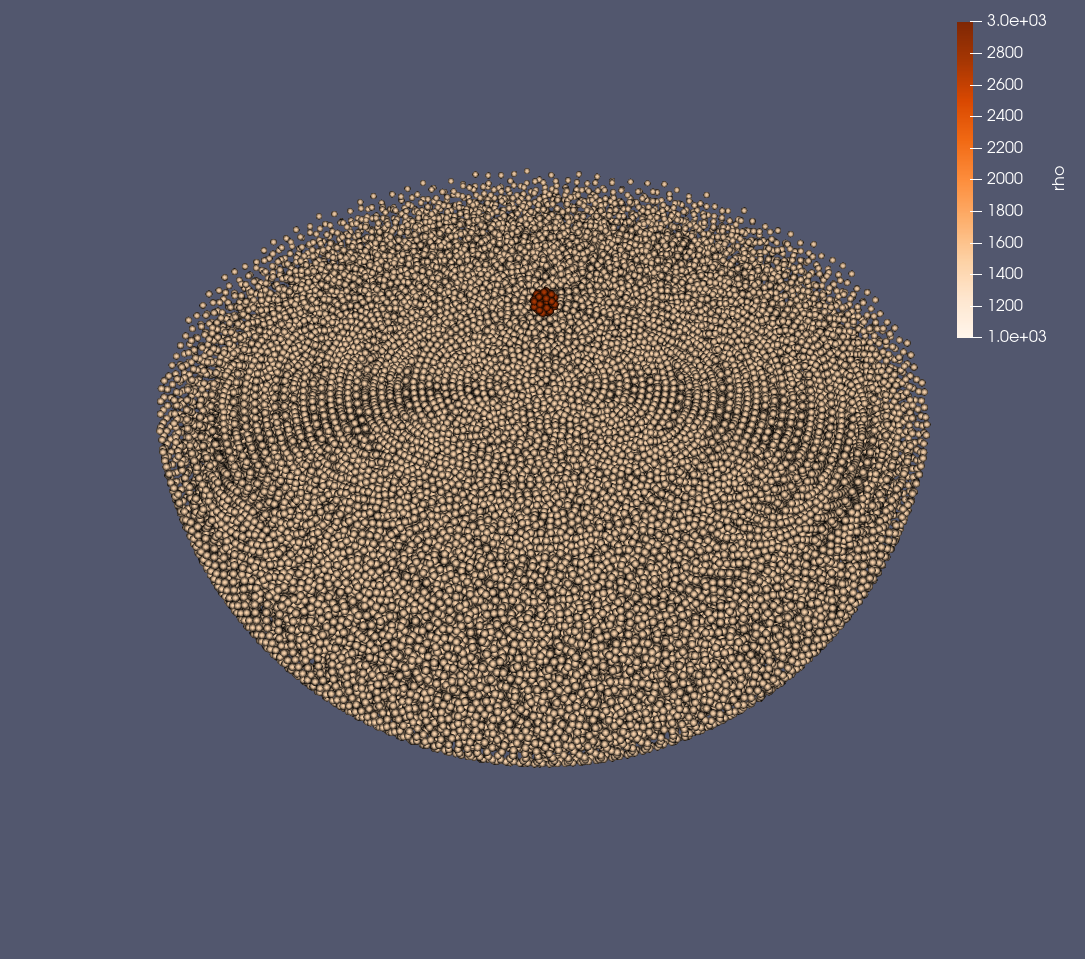
\includegraphics[width=\textwidth]{impact_start.png}
    \caption{start of example simulation}
    \label{fig:impact_start}
\end{figure}

\begin{figure}[H]
    \centering
    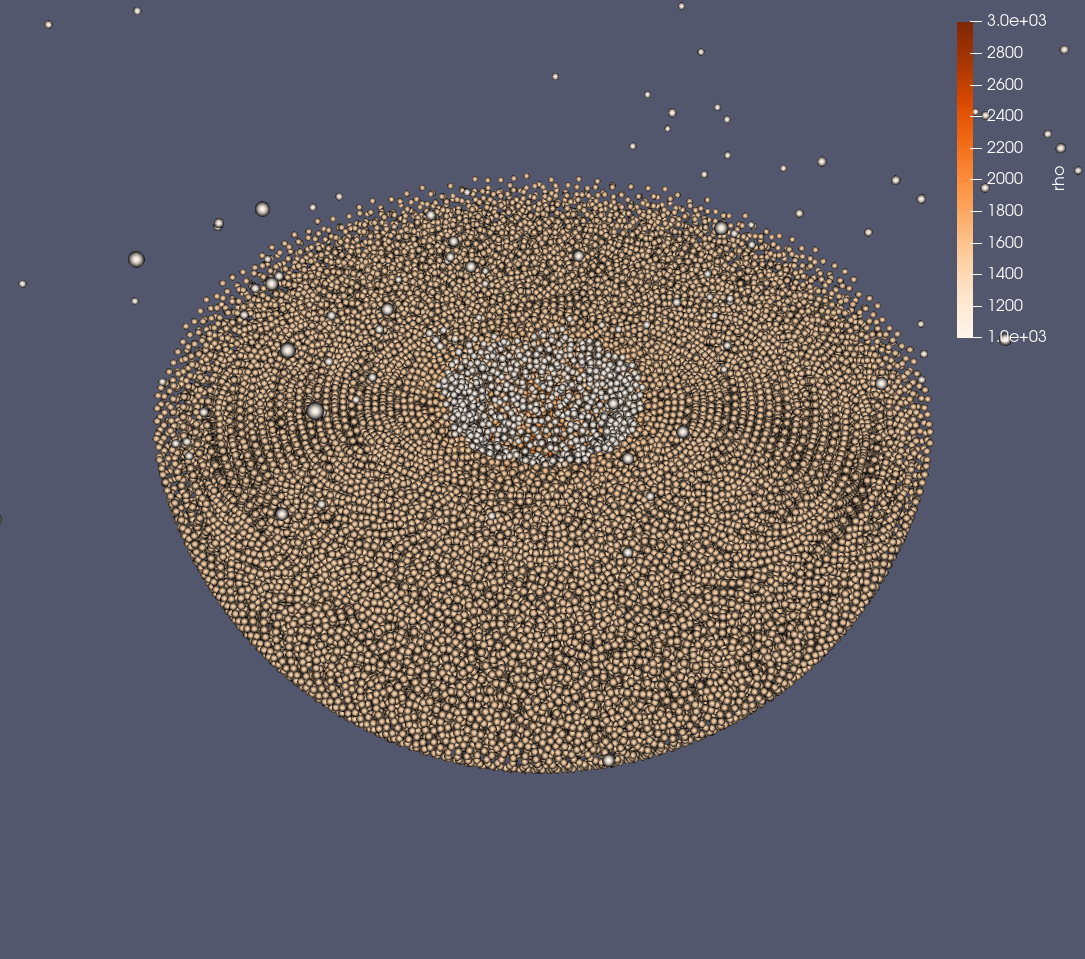
\includegraphics[width=\textwidth]{impact_end.png}
    \caption{end of example simulation}
    \label{fig:impact_end}
\end{figure}

\subsubsection{Material parameters} \label{sect:material_parameters}

\begin{table}
    \centering
    \begin{tabular}{ |l|l|l|l| }
        \hline
        \multicolumn{2}{|c|}{}                & Target                  & Projectile                                                          \\
        \hline
        \multirow{10}{*}{Tillotson EOS}       & $\rho_0$                & 2.86 $\cdot 10^3 g\cdot cm^{-3}$ & 2.70 $\cdot 10^3 g\cdot cm^{-3}$ \\
                                              & $A_T$                   & 2.67 $\cdot 10^{10}$ Pa          & 7.52 $\cdot 10^{10}$ Pa          \\
                                              & $B_T$                   & 2.67 $\cdot 10^{10}$ Pa          & 6.50 $\cdot 10^{10}$ Pa          \\
                                              & $E_0$                   & 4.87 $\cdot 10^8$ $Jkg^{-1}$     & 5.00 $\cdot 10^6$ $Jkg^{-1}$     \\
                                              & $E_{iv}$                & 4.72 $\cdot 10^6$ $Jkg^{-1}$     & 3.00 $\cdot 10^6$ $Jkg^{-1}$     \\
                                              & $E_{cv}$                & 1.82 $\cdot 10^7$ $Jkg^{-1}$     & 1.39 $\cdot 10^7$ $Jkg^{-1}$     \\
                                              & $a_T$                   & 0.5                              & 0.5                              \\
                                              & $b_T$                   & 1.5                              & 1.63                             \\
                                              & $\alpha_T$              & 5.0                              & 5.0                              \\
                                              & $\beta_T$               & 5.0                              & 5.0                              \\ \hline
        \multirow{7}{*}{Porosity}             & $\alpha_0$              & \textbf{varying}                 & not porous                       \\
                                              & $p_{elastic}$           & 1.0 $\cdot 10^6$ Pa              & not porous                       \\
                                              & $p_{transition}$        & 6.8 $\cdot 10^7$ Pa              & not porous                       \\
                                              & $p_{compacted}$         & 2.13 $\cdot 10^8$ Pa             & not porous                       \\
                                              & $\alpha_e$              & 4.64                             & not porous                       \\
                                              & $\alpha_t$              & 1.90                             & not porous                       \\
                                              & $c_s$                   & 100.0 $m\cdot s^{-1}$            & not porous                       \\ \hline
        \multirow{6}{*}{Strength}             & cohesive strength $Y_c$ & \textbf{varying}                 & 1.0 $\cdot 10^9$ Pa              \\
                                              & $\alpha_{intact}$       & 0.982793 rad                     & 0 rad                            \\
                                              & $\alpha_{damaged}$      & 0.540419 rad                     & 0 rad                            \\
                                              & shear modulus $\mu$     & 2.27 $\cdot 10^{10}$ Pa          & 2.69 $\cdot 10^{10}$ Pa          \\
                                              & bulk modulus $K_0$      & 2.67 $\cdot 10^{10}$ Pa          & 5.23 $\cdot 10^{10}$ Pa          \\
                                              & shear strength $Y_M$    & 3.5 $\cdot 10^9$ Pa              & 2.76 $\cdot 10^8$ Pa             \\ \hline
        \multirow{2}{*}{Fragmentation}        & Weibull m               & 16                               & no damage                        \\
                                              & Weibull k               & 1.0 $\cdot 10^{61}$              & no damage                        \\ \hline
        \multirow{2}{*}{Artificial viscosity} & $\alpha$                & 1.0                              & 1.0                              \\
                                              & $\beta$                 & 2.0                              & 2.0                              \\ \hline
        \hline
    \end{tabular}
    \caption{Material parameters for basalt target and aluminium Impactor}
    \label{tab:material_parameters}
\end{table}

- variable smoothing length min 0.1 bis max 10.0
- rholimit 0.95